\section{Bitcoin Reorg Depth Reaction}
\label{app:reorg}

Section~\ref{subsec:formal-invariants} states a threat-model boundary --
safety is modeled given Bitcoin reorganizations no deeper than a
configurable finality depth $K_{\text{DEEP\_FINALITY}}$ -- as a precondition of the formal result. This appendix tests the
implementation at and beyond that boundary with forced Bitcoin
reorganizations, each confirmed from the resulting block hashes, at five
depths in one seven-validator run: \{1, 2, 3, 5, 15\}, with $K_{\text{DEEP\_FINALITY}}{=}2$ and
a suspicious-state threshold of 5.

\begin{figure}[h]
\centering
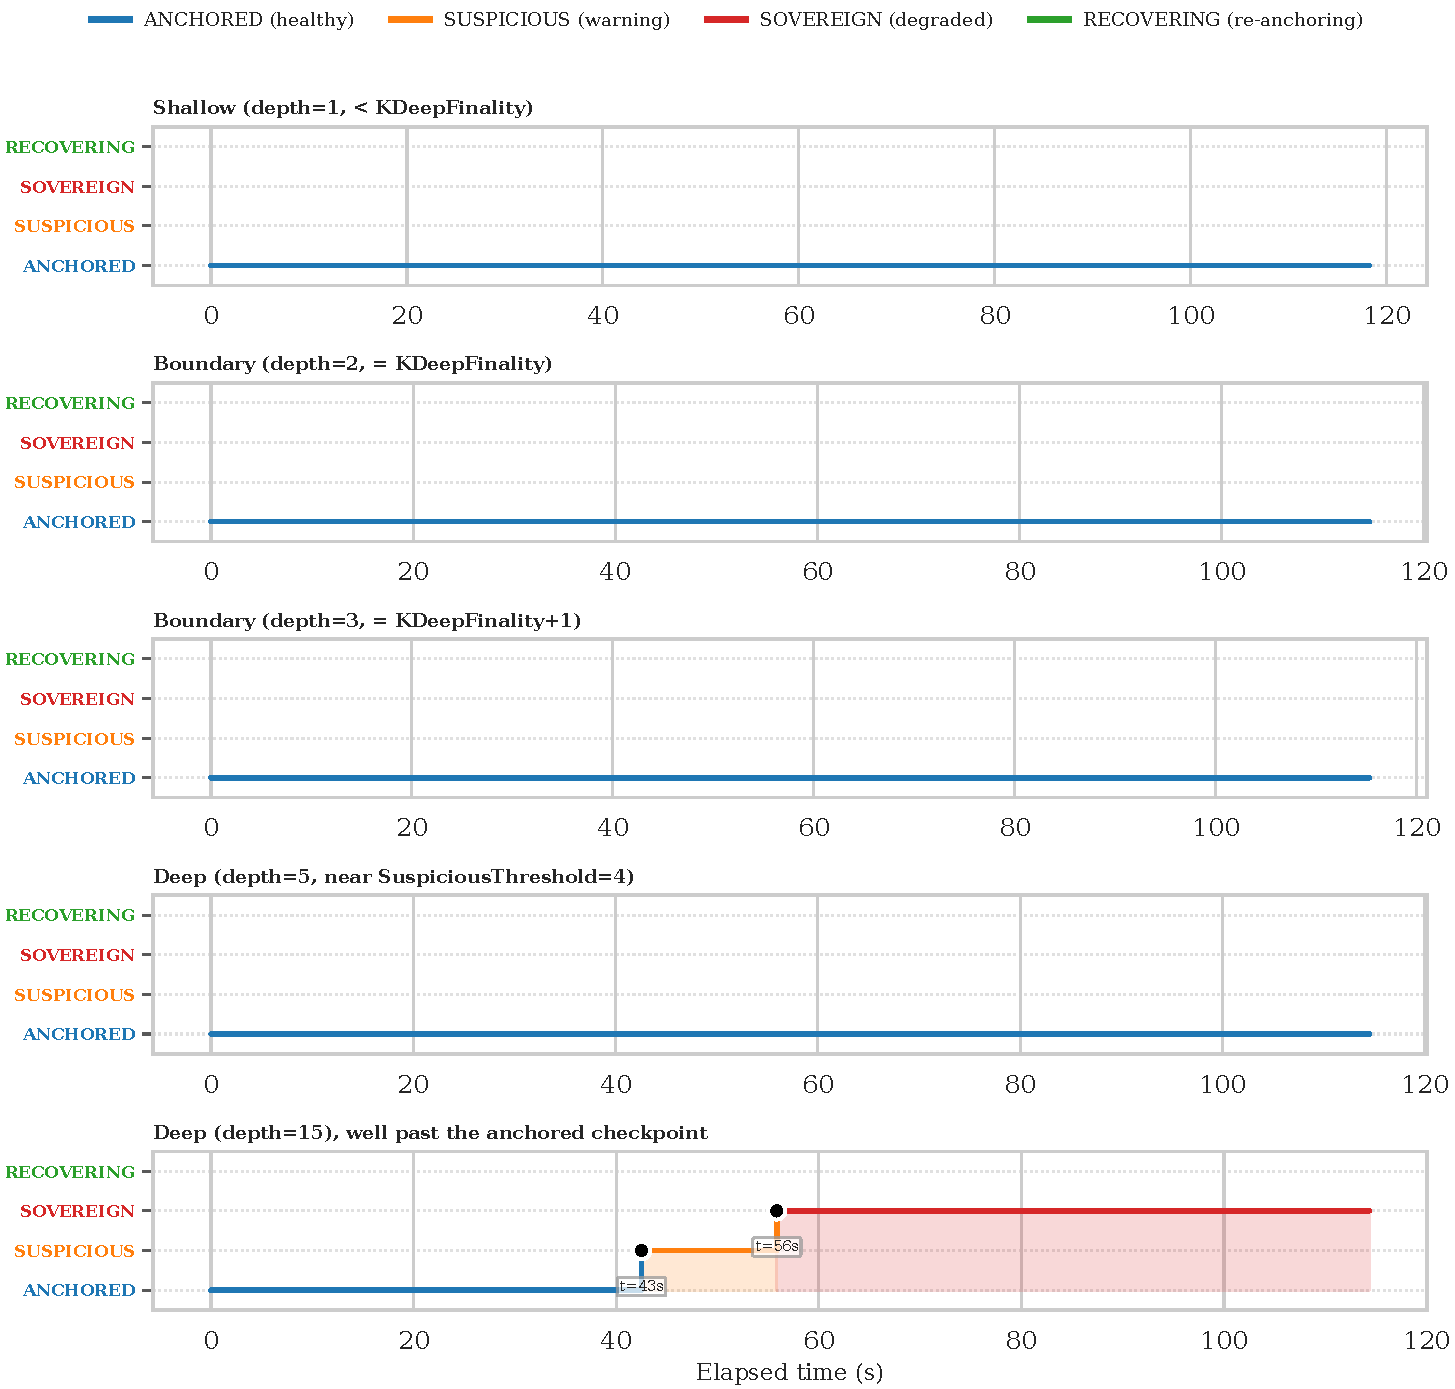
\includegraphics[trim=0 0 0 25pt, clip, width=\linewidth]{figures/figure8_reorg_depth_reaction_live.pdf}
\caption{FSM reaction to Bitcoin reorgs at five depths, one trial per
depth, seven-validator testbed. All 7 validators agree at every one of 181 polled
rounds per trial (1{,}267 samples total, 0 RPC errors).}
\label{fig:reorg}
\end{figure}

\FloatBarrier

Table~\ref{tab:reorg} summarizes the result. Depths 1--5 all orphan real,
independently-confirmed blocks, yet none of them trip the FSM within the
observation window: all 7 validators stay \textsc{Anchored} throughout. At
depth~15, all 7 validators transition \textsc{Anchored}$\to$\textsc{Suspicious}
at $t{=}43$\,s and $\to$\textsc{Sovereign} at $t{=}56$\,s, in lockstep. This
path rules out a direct critical-condition jump: the FSM's \textsc{Anchored}
branch bypasses \textsc{Suspicious} entirely when the committed certificate's
anchor-reverification flag is set, but the observed path instead passes
through \textsc{Suspicious}, and the suspicious-duration counter reached 23 of
the 24-block escalation bound ($\mathrm{MaxSuspiciousTime}$) in the last
sample before the \textsc{Sovereign} transition. The depth-15 reaction is
attributable to this duration-based escalation, not to anchor re-verification
failing.

\begin{table}[h]
\caption{FSM Reaction to Real Bitcoin Reorgs by Depth}
\label{tab:reorg}
\centering
\scriptsize
\begin{tabular}{@{}p{0.16\linewidth}p{0.24\linewidth}p{0.44\linewidth}@{}}
\toprule
\textbf{Depth} & \textbf{Reorg confirmed?} & \textbf{FSM reaction} \\
\midrule
1 (below $K_{\text{DEEP}}$) & N/A (too shallow) & Stays \textsc{Anchored} \\
2 ($=K_{\text{DEEP}}$)      & Yes & Stays \textsc{Anchored} \\
3 ($=K_{\text{DEEP}}{+}1$)  & Yes & Stays \textsc{Anchored} \\
5                           & Yes & Stays \textsc{Anchored} (within window) \\
15 (past checkpoint)        & Yes & \textsc{Suspicious}~(43s) $\to$ \textsc{Sovereign}~(56s) \\
\bottomrule
\end{tabular}
\end{table}

The crossover between depth~5 (no reaction) and depth~15 (reaction) was
not swept at finer granularity. Whether anchor re-verification ever set the
anchor-reverification flag during this run is not established by the
available logs -- the per-validator sensor value was not captured, only the
committed FSM state and suspicious-duration counter. The data that is
available shows the depth-15 escalation came from the suspicious-duration
bound, not from a direct critical-condition jump.

\FloatBarrier
